\documentclass[a4paper,12pt]{report}

\usepackage{alltt, fancyvrb, url}
\usepackage{graphicx}
\usepackage{subfigure}
\usepackage{wrapfig}
%\usepackage{algorithmic}
\usepackage[utf8]{inputenc}
\usepackage{fontenc}
\usepackage{amsthm}
\usepackage[english]{babel}
%stmaryrd,algorithm
\usepackage{amsmath,mathtools}
\usepackage{amssymb}
% Remove option to use English naming
\usepackage[english]{cleveref}


\title{Supervised Project ``Bicriteria Paths Problem''}
 
\author{Andrea Rossolini}
\date{\today}


\begin{document}
 
\maketitle

\begin{abstract}
In this paper I analyze a \textit{pathfinding} problem starting from a classical shortest path problem and then, after several optimization, going to resolve a graph that utilizes two static weights on his arches, considering the most full satisfying set of solutions.

As is known, Dijkstra's algorithm is most widely used to solve routing problems; in fact is very easy to create an implementation that attempts to find the best path in a classical weighted graph. So I will focus on the operations of optimization.
%
The most important part of the paper is the one that analyze the paths of a graph with two weights for each arches of it, one value represent the distance (also present in the monocriteria problem) and the other represent the danger of that arch. So the implementation will find not only the shortest and safest path, but also all the paths (not dominated) that take intermediate values. Two different algorithms will be shown for the analysis of the bicriteria problem.
\end{abstract}

\tableofcontents

\chapter{Introduction}
Dijkstra's algorithm, as already mentioned above, is widely used to find shortest path in routing problems that's use graphs with not-negative, static values. But this algorithm takes into consideration only one "dimension" of costs; for example, to calculate a path from the source node to the destination, distance is the result of adding up the length between two nodes segment by segment.
%
But the problem faced in our study considers two criteria for choosing the wanted path: the first cost defines the distance, while the second one represent the danger. So, the problem with Dijkstra is that we will found a path very short, but very dangerous, or vice versa. Concerning multicriteria shortest path problem is intended to determine a path that optimizes the costs from a source to the target, but, in general, there is no a single optimal solution, so the goal of this project is to determinate a set of feasible and not-dominated solution, founding different paths 
based on the two criteria, so is not sufficient minimizing distance or danger, but the relations between this two values.
\vspace{5mm}

\begin{figure}
	\centering
	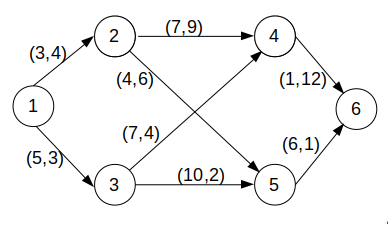
\includegraphics[width=\linewidth]{img/exampleGraph1}
	\caption{Graph example.}
	\label{fig:graphExample}
\end{figure}

\begin{table}[]
	\centering
	\begin{tabular}{|c|c|c|}
		\hline
		$p1$ & $1\to2\to4\to6$ & (11, 25) \\ \hline
		$p2$ & $1\to2\to5\to6$ & (13, 11)  \\ \hline
		$p3$ & $1\to3\to5\to6$ & (21, 6)  \\ \hline
		$p4$ & $1\to3\to4\to6$ & (13, 18)  \\ \hline
	\end{tabular}
	\caption{Graph's solution}
	\label{tab:graphExample}
\end{table}

In fig.\ref{fig:graphExample} is shown an example of a double criterion's routing. The nodes are labeled with numbers $\{1,2, ..., 6\}$ and the weights of the arches are represented as a pair of value (\textit{a, b}), where \textit{a} is distance and \textit{b} is danger.

In table \ref{tab:graphExample} are shown all the possible graph's iterations, $p1$ and $p3$ respectively the shortest and the safest paths, $p2$ is a not-dominated solution (it is longer than $p1$ but safer, more dangerous then $p3$, but, in this case, shorter) and $p4$ is a dominated path, so is useless to us.


 
\section{Mathematical formulation}

Let $G(N,A)$ denotes direct network which is composed of a finite set $N=\{0,1, \dots, n\}$ of nodes and a finite set $A \subseteq N\times N $, that represents the set of directed edges. Each arc can be denoted as an order pair $(i,j)$, where $i\in N$, $j \in N$ and both are two different nodes in $G(N,A)$.\\
Let define $c^k_{i,j}$ where $(i,j)\in A$ and $1\leq k \leq 2$ (because we are talking about a double criterion problem) represent the cost which we are referring to. We define two nodes in the graph: $s$ and $t$, where $s \in N$ and $t \in N$, these are respectively the \textit{source} and \textit{target} of which we want to find one or more paths.
%dei quali noi vogliamo trovare uno o più percorsi
We can qualify a path $p_{s,t}$ as a sequence  of  alternating nodes and arcs $p_{s,t} = \{s, (s, i_1), i_1, \dots, i_{l}, (i_l,t), t\}$.\\
So we said that each $c^k_{i,j}$ refers to one of the two costs of each arch $(i,j)$, therefore the total cost of the entire path can be represented in this way:\\

\begin{gather}(c^1(p_{s,t}), c^2(p_{s,t}))\end{gather}
\begin{gather}c^1(p_{s,t})=\sum_{(i,j)\in p}c^1_{i,j}\end{gather}
\begin{gather}c^2(p_{s,t})=\sum_{(i,j)\in p}c^2_{i,j}\end{gather}
Our purpose is to \textbf{minimize} the $(1.2)$ to find the shortest path or the $(1.3)$ to find the safest one.
%%%%%%%%%%%%%%%%%%%%%%%%%%%%%%%%%%%%%%%%%%%%%%%%%%%%%%%%%%%%%%%
%%SPOSTA LA DEFINIZIONE NELL'ANALISI DEL BICRITERIA ALGORITHM%%
%%%%%%%%%%%%%%%%%%%%%%%%%%%%%%%%%%%%%%%%%%%%%%%%%%%%%%%%%%%%%%%
\theoremstyle{definition}
\newtheorem{definition}{Definition}
\begin{definition}{Definition}
	Let $x, y$ be two distinct feasible path from a source $s$ to a target $t$. We say $x$ \emph{dominates} $y$ if and only of $c^k(x) \leq c^k(y)$ $\forall$ $k \in [1,2]$
\end{definition}
%AGGINGI ANCHE QUELLA SU PARETO FRONT SE RIESCI
%%%%%%%%%%%%%%%%%%%%

%\subsection*{Elementi positivi}
%\begin{itemize}
%	\item Si fornisce una descrizione in linguaggio naturale di ciò che il software dovrà fare.
%	\item Gli obiettivi sono spiegati con chiarezza, per punti.
%	\item Se il software è stato commissionato o è destinato ad un utente o compagnia specifici, il committente viene nominato.
%	\item Se vi sono termini il cui significato non è immediatamente intuibile, essi vengono spiegati.
%	\item Vengono descritti separatamente requisiti funzionali e non funzionali.
%\end{itemize} Inc.''\footnote{\url{http://aperturescience.com/}}




\chapter{Mono-criteria algorithms}

In this chapter will be explained the algorithms which concern the single criteria routing.
The analysis focuses on the evolution and optimization of the following algorithm, explaining some implementation choices.

\section{Dijkstra's algorithms}

Dijkstra's algorithm is a very famous algorithm used to find the shortest paths between nodes in a graph connected by arches with positive weights.\\
Different implementation of this algorithm are present in this paper, as follows are all explained.

\subsection{One to all}
This implementation is useful to find all the shortest path from a source node to each other graph's nodes. The starting node will save a dictionary where there is a key for each reached node and the respective value of distance.
It implement a \textit{pryority queue} so the complexity of this implementation is $O((|V|+|E|)\log(|V|))$ where $V$ is the number of vertices and $E$ the number of edges. In the worst case, so where $E>>V$, the time complexity is $(|E|\log(|V|))$.
Implementation's details are explained in the dedicated section.

\subsection{One to one}



\begin{itemize}
 \item Si mostrano pochi, mirati schemi UML dai quali si deduce con chiarezza quali sono le parti principali del software e come interagiscono fra loro.
 \item Si mette in evidenza se e come il pattern architetturale model-view-controller è stato applicato, anche con l'uso di un UML che mostri le interfacce principali ed i rapporti fra loro.
 \item Si discute se sia semplice o meno, con l'architettura scelta, sostituire in blocco la view senza toccare minimamente il controller. Va da sé che, se cambiare la UI si trasforma in un bagno di sangue che impatta controller o modello, il design architetturale non è stato fatto in modo adeguato.
\end{itemize}

\subsection*{Elementi negativi}
\begin{itemize}
 \item L'architettura è fatta in modo che sia impossibile riusare il modello per un software diverso che affronta lo stesso problema.
 \item L'architettura è tale che l'aggiunta di una funzionalità sul controller impatta pesantemente su view e/o modello.
 \item L'architettura è tale che la sostituzione in blocco della view impatta sul controller o, peggio ancora, sul modello.
 \item Si presentano UML caotici, difficili da leggere.
 \item Si presentano UML in cui sono mostrati elementi di dettaglio non appartenenti all'architettura, ad esempio includenti campi o con metodi che non interessano la parte di interazione fra le componenti principali del software.
 \item Si presentano schemi UML con classi (nel senso UML del termine) che ``galleggiano'' nello schema, non connesse, ossia senza relazioni con il resto degli elementi inseriti.
 \item Si presentano elementi di design di dettaglio, ad esempio tutte le classi e interfacce del modello o della view.
 \item Si discutono aspetti implementativi, ad esempio eventuali librerie usate oppure dettagli di codice.
\end{itemize}

\subsection*{Esempio}
L'architettura di GLaDOS segue il pattern architetturale ECB.
GLaDOS implementa l'interfaccia AI, ed è l'effettivo controller del sistema.
Essendo una intelligenza artificiale, è una classe attiva.
GLaDOS accetta la registrazione di Input ed Output.
Gli Input rappresentano delle nuove informazioni che vengono fornite all'IA, ad esempio delle modifiche nel valore di un sensore, oppure un comando da parte dell'operatore.
Questi input infatti forniscono eventi.
Ottenere un evento è un'operazione bloccante: chi la esegue resta in attesa di un effettivo evento.
Ogni volta che c'è un cambio alla situazione del soggetto, GLaDOS notifica i suoi Output, informandoli su quale sia la situazione corrente.

Con questa architettura, possono essere aggiunti un numero arbitrario di input ed output all'intelligenza artificiale.

In \Cref{img:goodarch} è esemplificato il diagramma UML architetturale.

\begin{figure}
\centering{}
%\includegraphics[width=\textwidth]{img/arch}
\caption{Schema UML architetturale di GLaDOS}
\label{img:goodarch}
\end{figure}


\section{Design dettagliato}

In questa sezione si possono approfondire alcuni elementi del design con maggior dettaglio.
%
Mentre ci attendiamo principalmente (o solo) interfacce negli schemi UML delle sezioni precedenti, in questa sezione è necessario scendere in maggior dettaglio presentando la struttura di alcune sottoparti rilevanti dell'applicazione.
%
È molto importante che, descrivendo un problema, quando possibile si mostri che non si è re-inventata la ruota ma si è applicato un design pattern noto.
%
È assolutamente inutile, ed è anzi controproducente, descrivere classe-per-classe (o peggio ancora metodo-per-metodo) com'è fatto il vostro software: è un livello di dettaglio proprio della documentazione dell'API (deducibile dalla Javadoc).

\textbf{È necessario che ciascun membro del gruppo abbia una propria sezione di design dettagliato, di cui sarà responsabile}.
%
Ciascun autore dovrà spiegare in modo corretto e giustamente approfondito (non troppo in dettaglio, non superficialmente) il proprio contributo.
%
È importante focalizzarsi sulle scelte che hanno un impatto positivo sul riuso, sull'estensibilità, e sulla chiarezza dell'applicazione.
%
Usare correttamente i design pattern in questa sezione è molto importante: se vengono utilizzati, si ha la garanzia che quanto fatto sia conforme allo stato dell'arte.

Esattamente come nessun ingegnere meccanico presenta un solo foglio con l'intero progetto di una vettura di Formula 1, ma molteplici fogli di progetto che mostrano a livelli di dettaglio differenti le varie parti della vettura e le modalità di connessione fra le parti, così ci aspettiamo che voi, futuri ingegneri informatici, ci presentiate prima una visione globale del progetto, e via via siate in grado di dettagliare le singole parti, scartando i componenti che non interessano quella in esame.
%
Per continuare il parallelo con la vettura di Formula 1, se nei fogli di progetto che mostrano il design delle sospensioni anteriori appaiono pezzi che appartengono al volante o al turbo, vuol dire che c'è qualche grosso problema di design.

\subsection*{Elementi positivi}

\begin{itemize}
	\item Ogni membro del gruppo discute le proprie decisioni di progettazione, ed in particolare le azioni volte ad anticipare possibili cambiamenti futuri (ad esempio l'aggiunta di una nuova funzionalità, o il miglioramento di una esistente).
	\item Si identificano ed utilizzano numerosi design pattern.
	\item Ogni membro del gruppo identifica i pattern utilizzati nella sua sottoparte.
	\item Si mostrano gli aspetti di design più rilevanti dell'applicazione, mettendo in luce la maniera in cui si è costruita la soluzione ai problemi descritti nell'analisi.
	\item Si tralasciano aspetti strettamente implementativi e quelli non rilevanti, non mostrandoli negli schemi UML (ad esempio, campi privati) e non descrivendoli.
	\item Si mostrano le principali interazioni fra le varie componenti che collaborano alla soluzione di un determinato problema.
	\item Ciascun design pattern identificato presenta una piccola descrizione del problema calato nell'applicazione, uno schema UML che ne mostri la concretizzazione nelle classi del progetto, ed una breve descrizione della motivazione per cui tale pattern è stato scelto.
	\item La divisione in package rispecchia l'architettura e consente di navigare facilmente il sorgente, dando brevi giustificazione alle scelte fatte.
\end{itemize}

\subsection*{Elementi negativi}
\begin{itemize}
	\item Il design del modello risulta scorrelato dal problema descritto in analisi.
	\item Si tratta in modo prolisso, classe per classe, il software realizzato.
	\item Non si presentano schemi UML esemplificativi.
	\item Non si individuano design pattern, o si individuano in modo errato (si spaccia per design pattern qualcosa che non lo è).
	\item Si producono schemi UML caotici e difficili da leggere, che comprendono inutili elementi di dettaglio.
	\item Si presentano schemi UML con classi (nel senso UML del termine) che ``galleggiano'' nello schema, non connesse, ossia senza relazioni con il resto degli elementi inseriti.
	\item Si tratta in modo inutilmente prolisso la divisione in package, elencando ad esempio le classi una per una.
	\item La divisione in package non rispecchia l'architettura, o è caotica.
\end{itemize}

% \subsection*{Esempio di buona suddivisione in package}
% L'applicazione è stata divisa in tre sottoparti logiche, come descritto nell'architettura: Model, Controller e Boundary. Maggiori dettagli sulle scelte fatte:
% \begin{itemize}
%  \item Radice: non avendo alcun dominio, abbiamo deciso di utilizzare il prefisso dell'Università, cui abbiamo aggiunto un nostro identificativo: \texttt{it.unibo.studentsgroup}. Inoltre, abbiamo aggiunto un suffisso che indentifica questo progetto, per cui tutti i package saranno prefissi da: \texttt{it.unibo.studentsgroup.thisapp}.
%  \item Abbiamo diviso l'applicazione in tre sottoparti logiche in architettura, la divisione in package le rispecchia: \texttt{.model}, \texttt{.control}, \texttt{.boundary}. 
%  \item Essendo la parte di gestione dell'I/O composta di molti sorgenti, abbiamo suddiviso \texttt{.boundary} in sottopackage: \texttt{.boundary.network} e \texttt{.boundary.local}.
%  \item All'interno del model il concetto di \texttt{InterfacciaMoltoUsata} è stato implementato da numerose classi diverse. Di conseguenza, abbiamo adottato un subpackage \texttt{.model.imoltousata} dove abbiamo organizzato tutte le implementazioni, rendendo più navigable il package \texttt{it.unibo.studentsgroup.thisapp.model}.
% \end{itemize}


\subsection*{Esempi di UML ben realizzati}

In questa sezione ci si concentrerà sugli aspetti di personalità e sul funzionamento del reporting di GLaDOS.

Il sistema per la gestione della personalità utilizza il pattern Strategy, come da \Cref{img:strategy}: le implementazioni di Personality possono essere modificate, e la modifica impatta direttamente sul comportamento di GLaDOS.

\begin{figure}
\centering{}
%\includegraphics[width=\textwidth]{img/strategy}
\caption{Rappresentazione UML del pattern Strategy per la personalità di GLaDOS}
\label{img:strategy}
\end{figure}

Sono state attualmente implementate due personalità, una buona ed una cattiva.
Quella buona restituisce sempre una torta valida, mentre quella cattiva restituisce sempre una torta.
Dato che le due personalità differiscono solo per il comportamento da effettuarsi in caso di percorso completato con successo, è stato utilizzato il pattern template method per massimizzare il riuso, come da \Cref{img:template}.
Il metodo template è onSuccess(), che chiama un metodo astratto e protetto makeCake().

\begin{figure}
\centering{}
%
\includegraphics[width=\textwidth]{img/template}
\caption{Rappresentazione UML dell'applicazione del pattern Template Method alla gerarchia delle Personalità}
\label{img:template}
\end{figure}

Per quanto riguarda il reporting, è stato utilizzato il pattern Observer per consentire la comunicazione uno-a-molti fra GLaDOS ed i sistemi di output.
Il suo utilizzo è esemplificato in \Cref{img:observer}

\begin{figure}
\centering{}
%\includegraphics[width=\textwidth]{img/observer}
\caption{Il pattern Observer è usato per consentire a GLaDOS di informare tutti i sistemi di output in ascolto}
\label{img:observer}
\end{figure}

\subsection*{Esempio di pessimo diagramma UML}

In \Cref{img:badarch} è mostrato il modo \textbf{sbagliato} di fare le cose.
%
Questo schema è fatto male perché:
\begin{itemize}
	\item È caotico.
	\item È difficile da leggere e capire.
	\item Vi sono troppe classi, e non si capisce bene quali siano i rapporti che intercorrono fra loro.
	\item Si mostrano elementi implementativi irrilevanti, come i campi e i metodi privati nella classe \texttt{AbstractEnvironment}.
	\item Se l'intenzione era quella di costruire un diagramma architetturale, allora lo schema è ancora più sbagliato, perché mostra pezzi di implementazione.
	\item Una delle classi, in alto al centro, galleggia nello schema, non connessa a nessuna altra classe, e di fatto costituisce da sola un secondo schema UML scorrelato al resto
	\item Le interfacce presentano tutti i metodi e non una selezione che aiuti il lettore a capire quale parte del sistema si vuol mostrare.
\end{itemize}


\begin{figure}
\centering{}
%\includegraphics[width=\textwidth]{img/badarch}
\caption{Schema UML mal fatto e con una pessima descrizione, che non aiuta a capire. Don't try this at home.}
\label{img:badarch}
\end{figure}


\chapter{Sviluppo}
\section{Testing automatizzato}

Il testing automatizzato è un requisito di qualunque progetto software che si rispetti, e consente di verificare che non vi siano regressioni nelle funzionalità a fronte di aggiornamenti.
%
Per quanto riguarda questo progetto è considerato sufficiente un test minimale, a patto che sia completamente automatico.
%
Test che richiedono l'intervento da parte dell'utente sono considerati \textit{negativamente} nel computo del punteggio finale.

\subsection*{Elementi positivi}

\begin{itemize}
 \item Si descrivono molto brevemente i componenti che si è deciso di sottoporre a test automatizzato.
 \item Si utilizzano suite specifiche (e.g. JUnit) per il testing automatico.
 \item Se sono stati eseguiti test manuali di rilievo, si elencano descrivendo brevemente la ragione per cui non sono stati automatizzati. Ad esempio, se tutto il team sviluppa e testa su uno stesso sistema operativo e si sono svolti test manuali per verificare, ad esempio, il corretto funzionamento dell'interfaccia grafica o di librerie native su altri sistemi operativi, può avere senso menzionare la cosa.
\end{itemize}

\subsection*{Elementi negativi}
\begin{itemize}
 \item Non si realizza alcun test automatico.
 \item La non presenza di testing viene aggravata dall'adduzione di motivazioni non valide.
 \item Si descrive un testing di tipo manuale in maniera prolissa.
 \item Si descrivono test effettuati manualmente che sarebbero potuti essere automatizzati, ad esempio scrivendo che si è usata l'applicazione manualmente.
\end{itemize}

\section{Metodologia di lavoro}

Ci aspettiamo, leggendo questa sezione, di trovare conferma alla divisione operata nella sezione del design di dettaglio, e di capire come è stato svolto il lavoro di integrazione.

\subsection*{Elementi positivi}

\begin{itemize}
	\item Si identifica con precisione il ruolo di ciascuno all'interno del gruppo, ossia su quale parte del progetto ciascuno dei componenti si è concentrato maggiormente.
	\item La divisione dei compiti è equa, ossia non vi sono membri del gruppo che hanno svolto molto più lavoro di altri
	\item La divisione dei compiti è coerente con quanto descritto nelle parti precedenti della relazione
	\item La divisione dei compiti è realistica, ossia le dipendenze fra le parti sviluppate sono minime
	\item Si identifica quale parte del software è stato sviluppato da tutti i componenti insieme.
	\item Si spiega in che modo si sono integrate le parti di codice sviluppate separatamente, evidenziando eventuali problemi. Ad esempio, una strategia è convenire sulle interfacce da usare (ossia, occuparsi insieme di stabilire l'architettura) e quindi procedere indipendentemente allo sviluppo di parti differenti. Una possibile problematica potrebbe essere una dimenticanza in fase di design architetturale che ha costretto ad un cambio e a modifiche in fase di integrazione. Una situazione simile è la norma nell'ingegneria di un sistema software non banale, ed il processo di progettazione top-down con raffinamento successivo è il così detto processo ``a spirale''.
	\item Si descrive in che modo è stato impiegato il DVCS.
\end{itemize}

\subsection*{Elementi negativi}
\begin{itemize}
	\item Non si chiarisce chi ha fatto cosa.
	\item C'è discrepanza fra questa sezione e le sezioni che descrivono il design dettagliato.
	\item Tutto il progetto è stato svolto lavorando insieme invece che assegnando una parte a ciascuno.
	\item Non viene descritta la metodologia di integrazione delle parti sviluppate indipendentemente.
	\item Uso superficiale del DVCS.
\end{itemize}

\section{Note di sviluppo}

Questa sezione, come quella riguardante il design dettagliato va svolta \textbf{singolarmente da ogni membro del gruppo}.

Ciascuno dovrà mettere in evidenza eventuali particolarità del suo metodo di sviluppo, ed in particolare:
\begin{itemize}
	\item Elencare le feature avanzate del linguaggio Java che sono state utilizzate. Le feature di interesse possono essere, ad esempio:
	\begin{itemize}
		\item Uso avanzato dei generici (ad esempio costruzione di nuovi tipi generici, e uso di generici bounded)
		\item Uso delle lambda expressions
		\item Uso degli stream, degli optional o di altri costrutti monadici
		\item Uso della reflection
		\item Uso di parti di libreria non spiegate a lezione (networking, JavaScript via Nashorn, eccetera...)
	\end{itemize}
	Si faccia molta attenzione a non scrivere banalità, elencando qui features di tipo ``core'', come le eccezioni, o le inner class.
	\item Descrivere eventuali approfondimenti fatti rispetto a quanto trattato nel corso (ad esempio l'utilizzo di un logger, o l'accesso alla rete, o l'uso di librerie grafiche particolari)
	\item Descrivere le librerie utilizzate nella propria parte di progetto. Si ricorda che l'utilizzo di librerie è valutato \emph{positivamente}.
	\item Sviluppo di algoritmi particolarmente interessanti \emph{non forniti da alcuna libreria}
\end{itemize}

In questa sezione è anche bene evidenziare eventuali pezzi di codice scopiazzati da Internet o da altri progetti (pratica che tolleriamo ma che non raccomandiamo).

\subsection*{Elementi positivi}

\begin{itemize}
	\item Si elencano gli aspetti avanzati di linguaggio che sono stati impiegati
	\item Si elencano le librerie che sono state utilizzate
	\item Si descrivono aspetti particolarmente complicati o rilevanti relativi all'implementazione, ad esempio, in un'applicazione performance critical, un uso particolarmente avanzato di meccanismi di caching, oppure l'implementazione di uno specifico algorigmo.
	\item Se si è utilizzato un particolare algoritmo, se ne cita la fonte originale. Ad esempio, se si è usato Mersenne Twister per la generazione dei numeri random, si cita \cite{mersenne}.
	\item Si identificano parti di codice prese da altri progetti, dal web, o comunque scritte in forma originale da altre persone. In tal senso, si ricorda che agli ingegneri non è richiesto di re-inventare la ruota continuamente: se ci cita debitamente la sorgente è tollerato fare uso di di snippet di codice per risolvere velocemente problemi non banali. Nel caso in cui si usino snippet di codice di qualità discutibile, oltre a menzionarne l'autore originale si invitano gli studenti ad adeguare tali parti di codice agli standard e allo stile del progetto. Contestualmente, si fa presente che è largamente meglio fare uso di una libreria che copiarsi pezzi di codice: qualora vi sia scelta, si preferisca la prima via.
\end{itemize}

\subsection*{Elementi negativi}
\begin{itemize}
	\item Si elencano feature core del linguaggio invece di quelle segnalate.
	\item Si descrivono aspetti di scarsa rilevanza, o si scende in dettagli inutili.
	\item Sono presenti parti di codice sviluppate originalmente da altri che non vengono debitamente segnalate. In tal senso, si ricorda agli studenti che i docenti hanno accesso a tutti i progetti degli anni passati, a Stack Overflow, ai principali blog di sviluppatori ed esperti Java e ai blog dedicati allo sviluppo di soluzioni e applicazioni (inclusi blog dedicati ad Android e allo sviluppo di videogame). Conseguentemente, è \emph{molto} conveniente \emph{citare} una fonte ed usarla invece di tentare di spacciare per proprio il lavoro di altri.
\end{itemize}

\chapter{Commenti finali}

In quest'ultimo capitolo si tirano le somme del lavoro svolto e si delineano eventuali sviluppi futuri.

\section{Autovalutazione e lavori futuri}

\subsection*{Cosa scrivere}

\textbf{È richiesta una sezione per ciascun membro del gruppo}.
%
Ciascuno dovrà autovalutare il proprio lavoro, elencando i punti di forza e di debolezza in quanto prodotto.
Si dovrà anche cercare di descrivere \emph{in modo quanto più obiettivo} il proprio ruolo all'interno del gruppo.
Si ricorda, a tal proposito, che ciascuno studente è responsabile solo della propria sezione: non è un problema se ci sono opinioni contrastanti, a patto che rispecchino effettivamente l'opinione di chi le scrive.
Nel caso in cui si pensasse di portare avanti il progetto, ad esempio perché effettivamente impiegato, o perché sufficientemente ben riuscito da poter esser usato come dimostrazione di esser capaci progettisti, si descriva brevemente verso che direzione portarlo.

\section{Difficoltà incontrate e commenti per i docenti}

Questa sezione, opzionale, può essere utilizzata per segnalare ai docenti eventuali problemi o difficoltà incontrate nel corso o nello svolgimento del progetto, può essere vista come una seconda possibilità di valutare il corso (dopo quella offerta dalle rilevazioni della didattica) avendo anche conoscenza delle modalità e delle difficoltà collegate all'esame, cosa impossibile da fare usando le valutazioni in aula per ovvie ragioni di tempistiche.
%
È possibile che alcuni dei commenti forniti vengano utilizzati per migliorare il corso in futuro: sebbene non andrà a vostro beneficio, potreste fare un favore ai vostri futuri colleghi.
%
Ovviamente il contenuto della sezione non impatterà il voto finale.

\appendix
\chapter{Guida utente}

Capitolo in cui si spiega come utilizzare il software. Nel caso in cui il suo uso sia del tutto banale, tale capitolo può essere omesso.

\subsection*{Elementi positivi}

\begin{itemize}
 \item Si istruisce in modo semplice l'utente sull'uso dell'applicazione, eventualmente facendo uso di schermate e descrizioni.
\end{itemize}

\subsection*{Elementi negativi}
\begin{itemize}
 \item Si descrivono in modo eccessivamente minuzioso tutte le caratteristiche, anche minori, del software in oggetto.
 \item Manca una descrizione che consenta ad un utente qualunque di utilizzare almeno le funzionalità primarie dell'applicativo.
\end{itemize}

\bibliographystyle{abbrv}
\bibliography{template}

\end{document}
